% Universal Optica Publishing Group format, using the author's supplied package.
% The official class is single-column; see README.md for the JOSA B length estimate.
\documentclass{optica-article}
\journal{opticajournal}
\articletype{Research Article}
\usepackage{amsmath,bm}
\usepackage{xr-hyper}
\usepackage{placeins,float,xurl}
\usepackage{lineno}
\linenumbers
\numberwithin{equation}{section}
% Generated by export-references.py; regenerate with make.
\newlabel{S-supp:sec:physical}{{S1}{S1}{Physical FWM normalisation}{section.1}{supplement.pdf}}
\newlabel{S-eq:fwm-system}{{S1}{S1}{Physical FWM normalisation}{equation.1}{supplement.pdf}}
\newlabel{S-eq:overlaps}{{S2}{S2}{Physical FWM normalisation}{equation.2}{supplement.pdf}}
\newlabel{S-eq:overlap-symms}{{S4}{S2}{Complex-envelope normalisation}{equation.4}{supplement.pdf}}
\newlabel{S-eq:T-def}{{S5}{S3}{Complex-envelope normalisation}{equation.5}{supplement.pdf}}
\newlabel{S-eq:u-v-A}{{S6}{S3}{Complex-envelope normalisation}{equation.6}{supplement.pdf}}
\newlabel{S-eq:physical-real-slice}{{S7}{S3}{Complex-envelope normalisation}{equation.7}{supplement.pdf}}
\newlabel{S-eq:uv-system}{{S10}{S4}{Complex-envelope normalisation}{equation.10}{supplement.pdf}}
\newlabel{S-eq:amplitude-phase-correspondence}{{S11}{S4}{Complex-envelope normalisation}{equation.11}{supplement.pdf}}
\newlabel{S-supp:sec:elliptic-data}{{S2}{S4}{Hamiltonian independence and elliptic reconstruction data}{section.2}{supplement.pdf}}
\newlabel{S-eq:prod-id}{{S12}{S5}{Scalar reduction and quartic chart}{equation.12}{supplement.pdf}}
\newlabel{S-eq:Q-uv}{{S13}{S5}{Scalar reduction and quartic chart}{equation.13}{supplement.pdf}}
\newlabel{S-eq:drho-sqrd-1}{{S14}{S5}{Scalar reduction and quartic chart}{equation.14}{supplement.pdf}}
\newlabel{S-eq:drho-sqrd-2}{{S15}{S5}{Scalar reduction and quartic chart}{equation.15}{supplement.pdf}}
\newlabel{S-eq:drho-sqrd-3}{{S16}{S5}{Scalar reduction and quartic chart}{equation.16}{supplement.pdf}}
\newlabel{S-eq:drho-sqrd-4}{{S17}{S5}{Scalar reduction and quartic chart}{equation.17}{supplement.pdf}}
\newlabel{S-eq:wp-4-to-3}{{S18}{S5}{Scalar reduction and quartic chart}{equation.18}{supplement.pdf}}
\newlabel{S-eq:rho-wp-1}{{S19}{S6}{Scalar reduction and quartic chart}{equation.19}{supplement.pdf}}
\newlabel{S-eq:dwp}{{S20}{S6}{Scalar reduction and quartic chart}{equation.20}{supplement.pdf}}
\newlabel{S-eq:g2-d}{{S21}{S6}{Scalar reduction and quartic chart}{equation.21}{supplement.pdf}}
\newlabel{S-eq:3-d}{{S22}{S6}{Scalar reduction and quartic chart}{equation.22}{supplement.pdf}}
\newlabel{S-eq:wp-points}{{S24}{S6}{Scalar reduction and quartic chart}{equation.24}{supplement.pdf}}
\newlabel{S-eq:dlog-u-v-zeta}{{S26}{S7}{Expanded logarithmic derivatives}{equation.26}{supplement.pdf}}
\newlabel{S-eq:zeta-dlog_sigma}{{S27}{S7}{Expanded logarithmic derivatives}{equation.27}{supplement.pdf}}
\newlabel{S-supp:sec:fs-proof}{{S3}{S7}{Detailed Frobenius--Stickelberger calculation}{section.3}{supplement.pdf}}
\newlabel{S-eq:fs-det-m}{{S28}{S7}{Detailed Frobenius--Stickelberger calculation}{equation.28}{supplement.pdf}}
\newlabel{S-eq:fs-det-start}{{S31}{S8}{Detailed Frobenius--Stickelberger calculation}{equation.31}{supplement.pdf}}
\newlabel{S-supp:subsec:fs-quasiperiod}{{S3.1}{S8}{The left hand side}{subsection.3.1}{supplement.pdf}}
\newlabel{S-eq:u-prod-is-one}{{S32}{S8}{The left hand side}{equation.32}{supplement.pdf}}
\newlabel{S-eq:quasi-sigma}{{S33}{S8}{The left hand side}{equation.33}{supplement.pdf}}
\newlabel{S-eq:exp-arg-is-one}{{S34}{S8}{The left hand side}{equation.34}{supplement.pdf}}
\newlabel{S-eq:nuj-sum-zero}{{S35}{S8}{The left hand side}{equation.35}{supplement.pdf}}
\newlabel{S-eq:roj-quasiperiod}{{S36}{S8}{The left hand side}{equation.36}{supplement.pdf}}
\newlabel{S-eq:waring-lagrange}{{S38}{S9}{The right hand side}{equation.38}{supplement.pdf}}
\newlabel{S-supp:sec:cubic}{{S4}{S10}{When quartic terms cancel through special parameter values}{section.4}{supplement.pdf}}
\newlabel{S-eq:u-v-cubic}{{S44}{S10}{When quartic terms cancel through special parameter values}{equation.44}{supplement.pdf}}
\newlabel{S-eq:modal-power-cubic}{{S45}{S10}{When quartic terms cancel through special parameter values}{equation.45}{supplement.pdf}}
\newlabel{S-supp:sec:normalisation}{{S5}{S10}{FWM gauge, intermediate Hamiltonian and reconstruction}{section.5}{supplement.pdf}}
\newlabel{S-eq:duv_bar_j}{{S53}{S11}{Barred Hamiltonian and common-pole envelopes}{equation.53}{supplement.pdf}}
\newlabel{S-eq:dwp-bar}{{S55}{S11}{Barred Hamiltonian and common-pole envelopes}{equation.55}{supplement.pdf}}
\newlabel{S-eq:dwp-h-bar}{{S56}{S11}{Barred Hamiltonian and common-pole envelopes}{equation.56}{supplement.pdf}}
\newlabel{S-eq:u-v-bar}{{S58}{S12}{Barred Hamiltonian and common-pole envelopes}{equation.58}{supplement.pdf}}
\newlabel{S-subsec:transform-domain}{{S5.3}{S12}{Physical-field reconstruction}{subsection.5.3}{supplement.pdf}}
\newlabel{S-supp:sec:coupler}{{S6}{S12}{Coherent-coupler solution data and physical map}{section.6}{supplement.pdf}}
\newlabel{S-cc:eq:jensen}{{S61}{S12}{Physical model and Hamiltonian variables}{equation.61}{supplement.pdf}}
\newlabel{S-cc:eq:uv-to-jensen}{{S62}{S13}{Physical model and Hamiltonian variables}{equation.62}{supplement.pdf}}
\newlabel{S-cc:eq:physical-slice}{{S63}{S13}{Physical model and Hamiltonian variables}{equation.63}{supplement.pdf}}
\newlabel{S-cc:eq:ham-uv}{{S64}{S13}{Conserved quantities and scalar reduction}{equation.64}{supplement.pdf}}
\newlabel{S-cc:eq:duv_j}{{S68}{S13}{Conserved quantities and scalar reduction}{equation.68}{supplement.pdf}}
\newlabel{S-cc:eq:uvj-gam-rho}{{S69}{S13}{Conserved quantities and scalar reduction}{equation.69}{supplement.pdf}}
\newlabel{S-cc:eq:power-conserved}{{S70}{S14}{Conserved quantities and scalar reduction}{equation.70}{supplement.pdf}}
\newlabel{S-cc:eq:Q-uv}{{S71}{S14}{Conserved quantities and scalar reduction}{equation.71}{supplement.pdf}}
\newlabel{S-cc:eq:drho-sqrd-1}{{S72}{S14}{Conserved quantities and scalar reduction}{equation.72}{supplement.pdf}}
\newlabel{S-cc:eq:drho-sqrd-2}{{S73}{S14}{Conserved quantities and scalar reduction}{equation.73}{supplement.pdf}}
\newlabel{S-cc:eq:drho-sqrd-3}{{S74}{S14}{Conserved quantities and scalar reduction}{equation.74}{supplement.pdf}}
\newlabel{S-cc:eq:drho-sqrd-4}{{S75}{S14}{Conserved quantities and scalar reduction}{equation.75}{supplement.pdf}}
\newlabel{S-cc:eq:lambda-root}{{S76}{S14}{Conserved quantities and scalar reduction}{equation.76}{supplement.pdf}}
\newlabel{S-cc:sec:mode-power}{{S6.3}{S14}{Elliptic powers and envelope solution}{subsection.6.3}{supplement.pdf}}
\newlabel{S-cc:eq:rho-wp-1}{{S77}{S14}{Elliptic powers and envelope solution}{equation.77}{supplement.pdf}}
\newlabel{S-cc:eq:wp-points}{{S78}{S15}{Elliptic powers and envelope solution}{equation.78}{supplement.pdf}}
\newlabel{S-cc:eq:uv-wp}{{S79}{S15}{Elliptic powers and envelope solution}{equation.79}{supplement.pdf}}
\newlabel{S-cc:eq:dlog-u-v-rho}{{S80}{S15}{Elliptic powers and envelope solution}{equation.80}{supplement.pdf}}
\newlabel{S-cc:eq:dlog-u-v-zeta}{{S84}{S16}{Elliptic powers and envelope solution}{equation.84}{supplement.pdf}}
\newlabel{S-cc:eq:zeta-dlog_sigma}{{S85}{S16}{Elliptic powers and envelope solution}{equation.85}{supplement.pdf}}
\newlabel{S-cc:eq:u-v-quartic}{{S86}{S16}{Elliptic powers and envelope solution}{equation.86}{supplement.pdf}}
\newlabel{S-cc:eq:r1j-sum}{{S88}{S17}{Elliptic powers and envelope solution}{equation.88}{supplement.pdf}}
\newlabel{S-cc:eq:branch-asymmetry}{{S89}{S17}{Elliptic powers and envelope solution}{equation.89}{supplement.pdf}}
\newlabel{S-cc:app:fs-det-ham-proof}{{S6.4}{S17}{Coupler Hamiltonian product and FS representation}{subsection.6.4}{supplement.pdf}}
\newlabel{S-cc:eq:fs-det-start}{{S90}{S17}{Coupler Hamiltonian product and FS representation}{equation.90}{supplement.pdf}}
\newlabel{S-cc:eq:u-prod-is-one}{{S91}{S17}{Divisor and exponential normalisation}{equation.91}{supplement.pdf}}
\newlabel{S-cc:eq:quasi-sigma}{{S92}{S17}{Divisor and exponential normalisation}{equation.92}{supplement.pdf}}
\newlabel{S-cc:eq:exp-arg-is-one}{{S93}{S17}{Divisor and exponential normalisation}{equation.93}{supplement.pdf}}
\newlabel{S-cc:eq:nuj-sum-zero}{{S94}{S17}{Divisor and exponential normalisation}{equation.94}{supplement.pdf}}
\newlabel{S-cc:eq:roj-is-zeta}{{S95}{S17}{Divisor and exponential normalisation}{equation.95}{supplement.pdf}}
\newlabel{S-cc:eq:poly-interp}{{S97}{S18}{Polynomial and determinant comparison}{equation.97}{supplement.pdf}}
\newlabel{S-supp:sec:projection}{{S7}{S19}{Degenerate-FWM construction and projection matching}{section.7}{supplement.pdf}}
\newlabel{S-cc:eq:two-to-three-ratios-sig}{{S109}{S19}{Coupler-gauge details}{equation.109}{supplement.pdf}}
\newlabel{S-cc:eq:ubar-vbar-degfwm-system}{{S111}{S20}{Degeneration and rescaling}{equation.111}{supplement.pdf}}
\newlabel{S-cc:eq:projection-elimination}{{S119}{S21}{Invariant matching and lift solutions}{equation.119}{supplement.pdf}}
\newlabel{S-cc:eq:projection-product-sum}{{S120}{S21}{Invariant matching and lift solutions}{equation.120}{supplement.pdf}}
\newlabel{S-cc:eq:-ubar-vbar-sols-dfwm}{{S122}{S22}{Invariant matching and lift solutions}{equation.122}{supplement.pdf}}
\newlabel{S-supp:sec:spectral}{{S8}{S22}{Wronskians and polynomial spectral potentials}{section.8}{supplement.pdf}}
\newlabel{S-supp:subsec:fwm-ba}{{S8.1}{S22}{Four-mode normal-form envelopes}{subsection.8.1}{supplement.pdf}}
\newlabel{S-eq:tilde-ba-pair}{{S123}{S22}{Four-mode normal-form envelopes}{equation.123}{supplement.pdf}}
\newlabel{S-eq:ba-abel-condition}{{S124}{S22}{Four-mode normal-form envelopes}{equation.124}{supplement.pdf}}
\newlabel{S-eq:ba-wronskian}{{S125}{S23}{Four-mode normal-form envelopes}{equation.125}{supplement.pdf}}
\newlabel{S-eq:ba-lame}{{S126}{S23}{Four-mode normal-form envelopes}{equation.126}{supplement.pdf}}
\newlabel{S-supp:subsec:coupler-ba}{{S8.2}{S23}{Degenerate-FWM lift of the coupler}{subsection.8.2}{supplement.pdf}}
\newlabel{S-cc:eq:lifted-wronskian}{{S128}{S23}{Degenerate-FWM lift of the coupler}{equation.128}{supplement.pdf}}
\newlabel{S-cc:eq:lifted-lame}{{S129}{S23}{Degenerate-FWM lift of the coupler}{equation.129}{supplement.pdf}}
\newlabel{S-subsec:kronecker-ba}{{S8.3}{S24}{Kronecker and theta representations}{subsection.8.3}{supplement.pdf}}
\newlabel{S-eq:kronecker-kernel}{{S130}{S24}{Kronecker and theta representations}{equation.130}{supplement.pdf}}
\newlabel{S-eq:ba-kronecker-theta}{{S131}{S24}{Kronecker and theta representations}{equation.131}{supplement.pdf}}
\newlabel{S-supp:sec:numerics}{{S9}{S24}{Additional numerical details}{section.9}{supplement.pdf}}
\newlabel{S-eq:A-phi-u-v}{{S132}{S24}{Additional numerical details}{equation.132}{supplement.pdf}}
\newlabel{S-fig:case1-plot1}{{S1}{S26}{\textbf {A} real and \textbf {B} imaginary parts of the complex mode power $\mathcal {P}_j=u_j v_j$, and \textbf {C} real and \textbf {D} imaginary parts of the complex phase variable $\phi _j$, using the analytic solutions in \externaleqref {M-eq:u-v-quartic} (dashed lines) compared against numerical integration of the abstract system \eqref {eq:uv-system} (symbols)}{figure.1}{supplement.pdf}}
\newlabel{S-supp:subsec:projection-numeric}{{S9.2}{S27}{Independent numerical projection comparison}{subsection.9.2}{supplement.pdf}}
\newlabel{S-app:param-def-appendix}{{S10}{S27}{FWM parameter definitions in the original coordinates}{section.10}{supplement.pdf}}
\newlabel{S-app:init-conds}{{S11}{S28}{FWM initial condition relations}{section.11}{supplement.pdf}}
\newlabel{S-app:bar-coords-params}{{S12}{S28}{Parameter definitions in the bar coordinates}{section.12}{supplement.pdf}}
\newlabel{S-app:scaled-params}{{S13}{S29}{Scaled parameters in the tilde coordinates}{section.13}{supplement.pdf}}
\newlabel{S-app:case1-params}{{S14}{S30}{Parameters for Figure \ref {fig:case1-plot1}}{section.14}{supplement.pdf}}
\newlabel{S-tab:case1-init}{{S1}{S30}{Initial mode values in Figure \ref {fig:case1-plot1}}{table.1}{supplement.pdf}}
\newlabel{S-tab:case1-params}{{S2}{S30}{Parameter values in Figure \ref {fig:case1-plot1}}{table.2}{supplement.pdf}}
\newlabel{S-app:case2-params}{{S15}{S30}{Parameters for Figure \ref *{M-fig:case2-plot1}}{section.15}{supplement.pdf}}
\newlabel{S-tab:case2-init}{{S3}{S30}{Initial field amplitudes for Figure~\ref *{M-fig:case2-plot1}; $|A_j|^2$ is in watts}{table.3}{supplement.pdf}}
\newlabel{S-tab:case2-physical}{{S4}{S31}{Parameters for Figure~\ref *{M-fig:case2-plot1}; entries are rounded}{table.4}{supplement.pdf}}
\newlabel{S-cc:app:param-def-appendix}{{S16}{S31}{Coherent-coupler parameter definitions}{section.16}{supplement.pdf}}
\newlabel{S-cc:app:init-conds}{{S17}{S31}{Coherent-coupler initial condition relations}{section.17}{supplement.pdf}}

\newcommand{\externaleqref}[1]{\textup{(\ref*{#1})}}
\begin{document}
\title{Elliptic complex-envelope solutions and normal forms for four-wave mixing and coherent couplers}
\author{Graham Hesketh\authormark{*}}
\address{Independent researcher, United Kingdom}
\email{\authormark{*}gdh1e10@gmail.com}
\begin{abstract*}
We reconstruct exact complex envelopes for continuous-wave four-wave mixing in Weierstrass functions, exposing their zeros, poles and branching and identifying their genus-one Baker--Akhiezer factors.
This representation connects the optical solutions to elliptic spectral theory and makes visible the analytic multipliers used in two transformations of the full mode equations.
First, gauges and a local normalisation yield a parameter-free meromorphic four-wave-mixing system; within this class of square-root normalisations, the power-exchange equation keeps its form in the original propagation variable only at total interaction degree four.
Second, a degenerate member of that system projects onto a reciprocally gauged asymmetric coherent coupler, whose envelopes are reconstructed explicitly.
Numerical comparisons and symbolic checks validate representative solutions and transformations.
\end{abstract*}

\section{Introduction}
Four-wave mixing (FWM) and nonlinear coherent coupling provide optical settings in which conservation laws, elliptic functions and Hamiltonian dynamics can be studied together.
In nonlinear fibres, Kerr-mediated FWM supports wavelength conversion, parametric amplification, optical signal processing and quantum light generation \cite{agrawalNonlinearFiberOptics2019,marhicFiberOpticalParametric2007}, including amplitude regeneration \cite{bottrillOptimisationAmplitudeLimiters2016} and reconfigurable optical activation functions \cite{yangReconfigurableOpticalNonlinear2026}.
The coherent coupler describes power-dependent exchange between evanescently coupled Kerr waveguide modes \cite{jensenNonlinearCoherentCoupler1982}.

Elliptic solutions for continuous-wave FWM powers, including pump depletion, are established \cite{chenFourphotonParametricMixing1989,chenFourwaveMixingOptical1989}, together with closed-form phases involving elliptic integrals of the third kind \cite{marhicAnalyticSolutionsPhases2013}.
For symmetric Kerr couplers, Stokes-space and Duffing reductions determine the powers and phase-invariant field products \cite{dainoStabilityAnalysisNonlinear1985}, while individual phase shifts have been obtained for general two-input excitation \cite[Sections~2--5]{pengIntensitydependentPhaseShifts1990}.
Asymmetric couplers with unequal propagation constants and Kerr coefficients have been treated through conserved quantities, power-flow portraits and quadratures \cite[Section~3.B and Appendix~A]{snyderPhysicsNonlinearFiber1991}.
Elliptic power-transfer solutions for single-core excitation cover asymmetrically distributed Kerr nonlinearity \cite{karpierzNonlinearDirectionalCouplers1992} and linear mismatch with nonlinear asymmetry \cite{wangEffectsLinearMismatch2001}.
Active asymmetric couplers with gain and loss have also been studied \cite{kominisAsymmetricActiveCoupler2016}; the present optical models are conservative on their physical slices.

Hamiltonian approaches include classical and quantum reductions and solutions for a particular FWM Hamiltonian under a frequency-resonance condition \cite{odzijewiczIntegrableClassicalQuantum2020}.
Related reconstruction settings include degenerate FWM \cite{cappelliniThirdorderThreewaveMixing1991}, geometric-phase reconstruction in resonant three-wave interactions \cite{alberGeometricPhasesReduction1998}, and the swinging-spring reduction \cite{holmStepwisePrecessionResonant2002}.
Weierstrass envelope representations also occur in quadratic wave mixing and polarisation dynamics \cite{heskethGeneralComplexEnvelope2015}.

The established power and phase descriptions determine the complex fields within their models.
Reconstructing the envelopes through logarithmic derivatives and sigma functions makes their zeros, poles, branching and exponential factors explicit.
Their Baker--Akhiezer factors connect the optical solutions to elliptic spectral theory, while the remaining analytic multipliers suggest transformations of the full mode equations.

\subsection{Our contribution}
The contribution is the use of complex-envelope reconstruction to expose analytic data and establish relationships between complete mode equations.
The results developed here are:
\begin{enumerate}
\item Complex-envelope reconstruction and its genus-one Baker--Akhiezer structure (Section~\ref{sec:fwm-solution}). The sigma representation exhibits the zeros, poles and local exponents, separates the Baker--Akhiezer factors and their branching multipliers, and identifies the associated Lam\'e equation.
\item A local, form-preserving transformation of generic quartic FWM trajectories to one parameter-free meromorphic system (Section~\ref{sec:coord-transforms}). Total interaction degree four distinguishes preservation of the power-exchange equation within the stated class of square-root normalisations, and the complete transformed mode equations retain the interaction structure.
\item A nonlinear ratio projection from a degenerate member of that four-mode system onto a reciprocally gauged asymmetric coupler, with explicit matching of the conserved quantities (Section~\ref{cc:sec:coord-transforms}). The coupler envelope solution also identifies the role of self-phase asymmetry in complex-plane branching.
\end{enumerate}
The envelope representation supplies the analytic visibility used in the normalisation and projection, providing two applications of the solution's function-theoretic structure.
Section~\ref{sec:num-val} validates the solutions and projection numerically; Supplement~1 contains the expanded algebra, spectral identities, parameter data and Frobenius--Stickelberger representations.

\section{General FWM solution and Baker--Akhiezer structure}\label{sec:fwm-solution}
We reconstruct the complex FWM envelopes from the conservation laws to expose the analytic factors that generate the normalisation and projection in Sections~\ref{sec:coord-transforms} and \ref{cc:sec:coord-transforms}.

\subsection{Model and conservation laws}\label{sec:fwm-model}
We consider the scalar continuous-wave fibre model with pump depletion, self-phase and cross-phase modulation, and phase mismatch $\Delta k=-\beta_1-\beta_2+\beta_3+\beta_4$ \cite{agrawalNonlinearFiberOptics2019,stolenParametricAmplificationFrequency1982}.
The physical equations, overlap assumptions and explicit field normalisation are given in Supplement~1, Section~\ref*{S-supp:sec:physical}.
With independent complex Hamiltonian variables $u_j,v_j$, they lead to the system
\begin{align}
\frac{d}{d z} u_j{\left(z \right)} &= - \left({a}_{j} + \sum_{k=1}^{4} {a}_{j,k}\,u_k v_k \right) u_j + \prod\limits_{k=1, k \ne j}^{4} v_k, \notag \\
\frac{d}{d z} v_j{\left(z \right)} &= \left({a}_{j} + \sum_{k=1}^{4} {a}_{j,k}\,u_k v_k \right) v_j - \prod\limits_{k=1, k \ne j}^{4} u_k. \label{eq:uv-system}
\end{align}
with $a_{j,k}=a_{k,j}$ and $j=1,\ldots,4$.
On the physical fibre slice,
\begin{equation}
v_j=-is_j u_j^*,\qquad
u_jv_j=-is_j\frac{T^2}{\omega_j}|A_j|^2,
\qquad s_1=s_2=1,\quad s_3=s_4=-1.
\label{eq:physical-real-slice}
\end{equation}
where $T$ is the normalisation scale in \externaleqref{S-eq:T-def}.
The modal products are therefore scaled, purely imaginary optical powers on this slice.
For physical coefficients, $\sum_j a_j=i\Delta k$.
The canonical Hamiltonian is
\begin{align}
\label{eq:ham-uv}
H(u_1,\dots, u_4, v_1, \dots, v_4) &= -\sum_{j=1}^{4} a_{j}\, u_j v_j - \frac{1}{2}\,\sum_{j,k=1}^{4} a_{j,k}\, u_j v_j u_k v_k + \prod\limits_{j=1}^{4} u_j + \prod\limits_{j=1}^{4} v_j, \\
\frac{d}{d z} u_j{\left(z \right)} &= \frac{\partial H}{\partial v_j}, \\
\frac{d}{d z} v_j{\left(z \right)} &= -\frac{\partial H}{\partial u_j}, \\
\frac{d}{d z} H &= 0
\end{align}

The interaction products have a common contribution to every modal-product derivative:
\begin{equation}
\label{eq:duv_j}
\frac{d}{d z} u_j v_j = - \prod\limits_{k=1}^{4} u_k + \prod\limits_{k=1}^{4} v_k
\end{equation}

\begin{equation}
\label{eq:uvj-gam-rho}
u_j(z) v_j(z) = \gamma_j - \rho(z)
\end{equation}

The conserved differences are
\begin{equation}
\label{eq:power-conserved}
u_j(z) v_j(z) - u_k(z) v_k(z) = \gamma_j - \gamma_k.
\end{equation}

Choose $\sum_j\gamma_j=0$, so $\rho$ is minus the mean modal product.
With $C_j=u_jv_j-u_4v_4$ for $j=1,2,3$, the quantities $H,C_1,C_2,C_3$ are generically independent and in involution; the complexified system is holomorphically Liouville integrable \cite{arnoldMathematicalMethodsClassical1989}.
The independence argument and parameter/initial-data definitions are given in Supplement~1, Sections~\ref*{S-supp:sec:elliptic-data}, \ref*{S-app:param-def-appendix} and \ref*{S-app:init-conds}.

\subsection{Elliptic modal powers}\label{sec:mode-power}
The Hamiltonian supplies the sum of the two interaction products, while \eqref{eq:duv_j} supplies their difference.
Squaring their difference and subtracting the square of their sum leaves $-4\prod_j u_jv_j$, giving a scalar quartic directly from the conservation laws.
Define
\begin{align}
Q(u_1(z)v_1(z), \dots, u_4(z)v_4(z)) &= a_0 + \sum_{j=1}^{4} a_{j}\, u_j v_j + \frac{1}{2}\,\sum_{j,k=1}^{4} a_{j,k}\, u_j v_j u_k v_k  \notag  \\
& = \sum_{l=0}^{2}b_l\,\rho\left(z\right)^l \label{eq:Q-uv}
\end{align}
with $a_0=H$. Then
\begin{equation}
\rho'^2=Q(\rho)^2-4\prod_{j=1}^4(\gamma_j-\rho)
=\sum_{l=0}^4d_l\rho^l
=d_4\prod_{l=1}^4(\rho-\lambda_l).
\label{eq:drho-sqrd-3}
\end{equation}
For $d_4\ne0$ and a nonsingular elliptic curve $g_2^3-27g_3^2\ne0$, choose a simple root $\lambda_1$ and a local chart with nonzero denominators.
A shift by $\lambda_1$, inversion and an affine scaling give the Weierstrass solution
\begin{align}
\rho{\left(z \right)} &= {\lambda}_{1} + \frac{d_4}{- 4 w{\left(z \right)} \prod_{l=1}^{3} {\Omega}_{l}  + \frac{d_4}{3} \sum_{l=1}^{3} {\Omega}_{l} }, \label{eq:rho-wp-1} \\
\Omega_l &= \frac{1}{\lambda_{l+1} - \lambda_1}, \notag \\
\left(\frac{d}{d z} w{\left(z \right)}\right)^{2} &= 4\,w{\left(z \right)}^3 - g_2\,w{\left(z \right)} - g_3, \label{eq:dwp} \\
g_{2} &= {d}_{0} {d}_{4} - \frac{{d}_{1} {d}_{3}}{4} + \frac{{d}_{2}^{2}}{12}, \label{eq:g2-d} \\
g_{3} &= \frac{{d}_{0} {d}_{2} {d}_{4}}{6} - \frac{{d}_{0} {d}_{3}^{2}}{16} - \frac{{d}_{1}^{2} {d}_{4}}{16} + \frac{{d}_{1} {d}_{2} {d}_{3}}{48} - \frac{{d}_{2}^{3}}{216} \label{eq:3-d}
\end{align}
where $w(z)=\wp(z-z_0;g_2,g_3)$.
Fixing initial data still requires inversion of $\wp$; specifying both $\wp$ and $\wp'$ fixes the sheet, modulo the period lattice.
The points $z_0\pm z_1$ are the poles of $\rho$, and $\mu_j$ is selected by $\rho(\mu_j)=\gamma_j$, $\rho'(\mu_j)=Q(\gamma_j)$, so that $v_j$ vanishes there and $u_j$ vanishes at $2z_0-\mu_j$.
The sign of $\sqrt{d_4}$ fixes the $z_1$ convention.
Explicit signed-point data are given in \externaleqref{S-eq:wp-points} of Supplement~1.
The modal powers follow as
\begin{align}
u_j{\left(z\right)} v_j{\left(z\right)} &= \rho(\mu_j) - \rho(z) \notag \\
&= \frac{\wp'{\left(z_{1}\right)}}{ \sqrt{{d}_{4}} \left(\wp{\left(z_{1}\right)} - \wp{\left({\mu}_{j} - z_{0}\right)}\right)} - \frac{\wp'{\left(z_{1}\right)}}{\sqrt{{d}_{4}} \left(\wp{\left(z_{1}\right)} - \wp{\left(z - z_{0}\right)}\right) } \notag \\
&= \frac{\wp'{\left(z_{1}\right)} }{ \sqrt{{d}_{4}} \left(\wp{\left(z_{1}\right)} - \wp{\left({\mu}_{j}- z_{0}\right)}\right)} \frac{ \left(\wp{\left(z - z_{0}\right)} - \wp{\left({\mu}_{j} - z_{0}\right)}\right) }{ \left(\wp{\left(z - z_{0}\right)} - \wp{\left(z_{1}\right)}\right) }. \label{eq:uv-wp}
\end{align}


\subsection{Complex envelopes} \label{sec:mode-sols-u-v}

Having obtained the modal power solutions in the previous section, we now proceed to find solutions for the individual modes $u_j(z)$ and $v_j(z)$ themselves.
Direct substitution of \eqref{eq:ham-uv}, \eqref{eq:duv_j}, \eqref{eq:uvj-gam-rho}, and \eqref{eq:power-conserved} into \eqref{eq:uv-system} shows that the equations can be recast in terms of logarithmic derivatives:
\begin{align}
\frac{\frac{\mathrm{d}}{\mathrm{d}z} u_j{\left(z\right)}}{u_j{\left(z\right)}} &= \frac{1}{2}\frac{\rho'{\left(z \right)} - \rho'{\left({\mu}_{j} \right)}}{\rho{\left(z \right)} - \rho{\left({\mu}_{j} \right)}} + \rho{\left(z \right)} {\Lambda}_{1,j} + {\Lambda}_{0,j}, \notag \\
\frac{\frac{\mathrm{d}}{\mathrm{d}z} v_j{\left(z\right)}}{v_j{\left(z\right)}} &= \frac{1}{2}\frac{\rho'{\left(z \right)} + \rho'{\left({\mu}_{j} \right)}}{\rho{\left(z \right)} - \rho{\left({\mu}_{j} \right)}} - \rho{\left(z \right)} {\Lambda}_{1,j} - {\Lambda}_{0,j}, \label{eq:dlog-u-v-rho} \\
{\Lambda}_{0,j} &= - {a}_{j} - \frac{{\gamma}_{j}}{4} \sum\limits_{k,l=1}^{4} {a}_{k,l} - \sum_{k=1}^{4} {a}_{j,k} {\gamma}_{k} + \frac{1}{2}\sum_{k=1}^{4} {\gamma}_{k} \sum_{l=1}^{4} {a}_{k,l} + \frac{1}{2}\sum_{k=1}^{4} {a}_{k}, \\
{\Lambda}_{1,j} &= \sum_{k=1}^{4} {a}_{j,k} - \frac{1}{4}\sum\limits_{k,l=1}^{4}  {a}_{k,l},
\end{align}
where the right-hand side is expressed purely in terms of $\rho$ and its derivative $\rho'$.
This logarithmic derivative form is advantageous because it can be integrated directly to yield solutions in terms of Weierstrass $\sigma$ functions, as we now show.

Substitute the elliptic powers into these logarithmic derivatives and use
\begin{equation}
\frac{\wp'(x)}{\wp(x)-\wp(y)}=\zeta(x+y)+\zeta(x-y)-2\zeta(x),
\qquad \zeta(x)=\frac{d}{dx}\log\sigma(x).
\end{equation}
The result is a sum of zeta functions, whose integration gives sigma ratios and elementary exponential factors.
The expanded derivatives are recorded in Supplement~1, Section~\ref*{S-supp:sec:elliptic-data}.
Performing the integration and taking exponentials gives the first main result of this paper, the complete analytic solutions for the complex mode envelopes $u_j,v_j$ of continuous-wave four-wave mixing, without decomposition into amplitude and phase:
\begin{align}
u_j{\left(z\right)} &= \frac{\alpha_j\,\sqrt{W_j} \,\sigma{\left(z - 2 z_{0} + {\mu}_{j} \right)} \exp\left(z {r}_{0,j} + \log{\left(\frac{\sigma{\left(z - z_{0} + z_{1} \right)}}{\sigma{\left(z - z_{0} - z_{1} \right)}} \right)} {r}_{1,j}\right)}{\sqrt{\wp{\left(z_{1} \right)} - \wp{\left(z - z_{0} \right)}} \sigma{\left({\mu}_{j} - z_{0}\right)} \sigma{\left(z - z_{0} \right)}}, \notag \\[12pt]
v_j{\left(z\right)} &= \frac{\sqrt{W_j} \, \sigma{\left(z - {\mu}_{j} \right)} \exp\left(- z {r}_{0,j} - \log{\left(\frac{\sigma{\left(z - z_{0} + z_{1} \right)}}{\sigma{\left(z - z_{0} - z_{1} \right)}} \right)} {r}_{1,j} \right)}{\alpha_j\,\sqrt{\wp{\left(z_{1} \right)} - \wp{\left(z - z_{0} \right)}} \sigma{\left({\mu}_{j} - z_{0}\right)} \sigma{\left(z - z_{0} \right)}} \label{eq:u-v-quartic}
\end{align}
where roots and logarithms are continued consistently on a simply connected chart from the initial data at $z=0$, $\alpha_j$ is the integration constant that can be fixed by initial conditions to capture any phase offset between a mode and its conjugate, and the other constants are:
\begin{align}
W_j &= \gamma_j-\lambda_1, \\[6pt]
r_{0,j} &= {\Lambda}_{0,j} + {\Lambda}_{1,j} {\lambda}_{1} - \frac{2 \zeta{\left(z_{1} \right)} {\Lambda}_{1,j}}{\sqrt{{d}_{4}}} - \frac{\zeta{\left({\mu}_{j} - z_{0} - z_{1}\right)}}{2} - \frac{\zeta{\left({\mu}_{j} - z_{0} + z_{1}\right)}}{2}, \\[6pt]
r_{1,j} &= \frac{{\Lambda}_{1,j}}{\sqrt{{d}_{4}}}.
\end{align}
The four $\alpha_j$ are constrained: their product is fixed by $2\prod_j u_j(0)=\rho'(0)+Q(\rho(0))$.
Thus the continuous constants comprise three independent $\gamma_j$, the Hamiltonian, $z_0$, and three independent envelope constants, giving eight complex parameters, as required.
The definitions also give $\sum_j\Lambda_{1,j}=\sum_jr_{1,j}=0$, so the logarithmic factors cancel from the complete mode products.


% ---------- SECTION -------------
% --------------------------------

The Hamiltonian product relation has a four-point Frobenius--Stickelberger determinant representation, derived in Supplement~1, Section~\ref*{S-supp:sec:fs-proof} \cite{whittakerCourseModernAnalysis2021,frobeniusZurTheorieElliptischen1877}.

\subsection{Zeros, poles and branching}\label{sec:cubic-case}
For generic noncoincident arguments, the quartic envelope $u_j$ has local exponents $r_{1,j}-1/2$ and $-r_{1,j}-1/2$ at $z_0-z_1$ and $z_0+z_1$, respectively; those of $v_j$ are interchanged.
This follows by writing $x=z-z_0$, $\nu_j=\mu_j-z_0$ and
\begin{equation}
u_j(z)\propto e^{zr_{0,j}}\sigma(x+\nu_j)
\sigma(x+z_1)^{r_{1,j}-1/2}\sigma(x-z_1)^{-r_{1,j}-1/2}.
\end{equation}
Noninteger exponents yield branch points, with compatible local branches required.
The distinct coefficient regime $d_4=b_2^2-4=0$, $d_3\ne0$, has cubic modal powers, but generically essential-singular envelopes because their reconstruction contains $\exp[-4\Lambda_{1,j}\zeta(z-z_0+z_1)/d_3]$.
The complete cubic formulas are given in Supplement~1, Section~\ref*{S-supp:sec:cubic}.
The FWM normal form in Section~\ref{sec:coord-transforms} belongs to the meromorphic subclass $d_4=0$, $\Lambda_{1,j}=0$, whose envelopes have the sigma-ratio structure identified in Section~\ref{sec:elliptic-structure}.

\subsection{Baker--Akhiezer structure of the envelopes}\label{sec:elliptic-structure}
Let $\Psi(x,a)$ denote the genus-one Baker--Akhiezer function in the plus-sign sigma convention,
\begin{equation}
\Psi(x,a)=\frac{\sigma(x+a)}{\sigma(x)\sigma(a)}e^{-x\zeta(a)},
\qquad a\notin\text{period lattice}.
\label{eq:ba-kronecker}
\end{equation}
This is the convention $a\mapsto-a$ relative to \cite[Eq.~(1.7)]{kricheverEllipticSolutionsNonlinear1994}.
For fixed $a$, $\Psi$ is meromorphic and quasiperiodic in $x$; in its spectral argument $a$ it has the prescribed exponential singularity at the origin of the elliptic curve.
These divisor and exponential data are the defining ingredients of the Baker--Akhiezer construction.

With $x=z-z_0$ and $\nu_j=\mu_j-z_0$, the sigma ratios in \eqref{eq:u-v-quartic} are
\begin{align}
\frac{\sigma(x+\nu_j)}{\sigma(x)\sigma(\nu_j)}
&=e^{x\zeta(\nu_j)}\Psi(x,\nu_j),\notag\\
\frac{\sigma(x-\nu_j)}{\sigma(x)\sigma(\nu_j)}
&=-e^{-x\zeta(\nu_j)}\Psi(x,-\nu_j).
\label{eq:general-ba-factors}
\end{align}
Thus the general FWM envelopes consist of Baker--Akhiezer factors multiplied by the explicit square-root, logarithmic and exponential factors in \eqref{eq:u-v-quartic}.
The square-root and logarithmic multipliers encode the branching described in Section~\ref{sec:cubic-case}.
All four pairs share one elliptic curve, and their spectral arguments obey $\sum_{j=1}^4\nu_j\equiv0$ modulo its period lattice: the elliptic product $\prod_j u_j$ has zeros at $x=-\nu_j$ and double poles at $x=\pm z_1$, so Abel's divisor condition fixes this sum.

The Baker--Akhiezer factors satisfy the one-gap Lam\'e equation
\begin{equation}
\frac{\partial^2\Psi(x,a)}{\partial x^2}
=[2\wp(x)+\wp(a)]\Psi(x,a),
\label{eq:general-ba-lame}
\end{equation}
with spectral parameter $\wp(a)$ \cite[Eq.~(1.9)]{kricheverEllipticSolutionsNonlinear1994}.
The same sigma-ratio and Abelian-exponential structure extends to higher genus; for example, the genus-two Baker function contains a shifted sigma ratio and second-kind Abelian integrals \cite[Eq.~(3.3)]{bradenBilinearRecurrencesAddition2005}.
The optical envelopes therefore make the divisor and exponential data of integrable-systems functions explicit.
The separation in \eqref{eq:general-ba-factors} now motivates two applications: removing the branching multipliers to obtain the FWM normal form in Section~\ref{sec:coord-transforms}, and constructing the coupler projection in Section~\ref{cc:sec:coord-transforms}.

\section{Normal form of four-wave mixing}\label{sec:coord-transforms}
We use the factors exposed in Section~\ref{sec:elliptic-structure} to construct a parameter-free meromorphic system while preserving the full four-mode interaction structure.
The construction acts locally on trajectories at fixed conserved quantities; the original parameters enter the transformed initial data and inverse reconstruction, and each target system is supplied with its Hamiltonian.
The denominator $\sqrt{\wp(z_1)-\wp(z-z_0)}$ in \eqref{eq:u-v-quartic} suggests a local mode normalisation, while its fractional-power factor suggests a reciprocal gauge.

\subsection{Gauge and local normalisation}\label{subsec:bar-coords}
Set $u_j=\hat u_j e^{-\phi_j}$, $v_j=\hat v_j e^{\phi_j}$ with $\sum_j\phi_j=0$.
The phases specified in Supplement~1, Section~\ref*{S-supp:sec:normalisation}, preserve all modal products, remove the mode-dependent logarithmic factors and give
\begin{align}
\frac{\mathrm{d}}{\mathrm{d}z} \hat{u}_j &= \left(b_1 - 2b_2\hat{u}_j \hat{v}_j \right) \frac{\hat{u}_j}{4} + \prod\limits_{k=1, k \ne j}^{4} \hat{v}_k \notag \\
\frac{\mathrm{d}}{\mathrm{d}z} \hat{v}_j &= -\left(b_1 - 2b_2\hat{u}_j \hat{v}_j\right) \frac{\hat{v}_j}{4} - \prod\limits_{k=1, k \ne j}^{4} \hat{u}_k \label{eq:uv-hat-system}
\end{align}

Here $b_1$ is constant on the chosen power leaf and $b_2$ depends only on the original coefficients.
For the local normalisation, put $\mathcal F(\rho)=\sum_l d_l\rho^l$ and choose a simple root $\lambda_1$ satisfying
\begin{equation}
\lambda_1\ne0,\qquad d_5=\mathcal F'(\lambda_1)\ne0,\qquad
q_1=Q(\lambda_1)\ne0.
\end{equation}
The root relation $q_1^2=4\prod_j(\gamma_j-\lambda_1)$ then ensures $\gamma_j-\lambda_1\ne0$ and $\chi=8q_1/d_5\ne0$.
Set $h(z)=\lambda_1d_5/(\lambda_1-\rho(z))$ and choose a simply connected chart on which $h$ is finite and nonzero.
The root branches are fixed compatibly by the initial data.
The next transformation is
\begin{align}
\hat{u}_j(z) &= 2 \sqrt{{\lambda}_{1} \left({\gamma}_{j} - {\lambda}_{1}\right)} \frac{\bar{u}_j(z) e^{-\theta_j z}}{\sqrt{h{\left(z \right)}}} \notag \\
\hat{v}_j(z) &= 2 \sqrt{{\lambda}_{1} \left({\gamma}_{j} - {\lambda}_{1}\right)}  \frac{\bar{v}_j(z) e^{\theta_j z} }{\sqrt{h{\left(z \right)}}} \notag \\
h{\left(z \right)} &= {d}_{5} - \sum_{l=1}^{4} \left({\gamma}_{l} - {\lambda}_{1}\right) \bar{u}_l \bar{v}_l = 4 {\lambda}_{1} \bar{u}_j \bar{v}_j - \frac{{\lambda}_{1}{d}_{5} }{{\gamma}_{j} - {\lambda}_{1}} \label{eq:hat-to-bar}
\end{align}
where the constants needed to evaluate the map are
\begin{align}
\chi&=\frac{8Q(\lambda_1)}{d_5},\qquad
\varsigma=\frac{Q(\lambda_1)}{2\sqrt{\prod_{k=1}^4(\gamma_k-\lambda_1)}}=\pm1,\notag\\
\theta_j&=\frac{Q(\lambda_1)}{2(\gamma_j-\lambda_1)}
+\frac{b_1}{4}+\frac{b_2(\gamma_j+\lambda_1)}{2}-\frac1\chi,
\qquad \sum_{j=1}^4\theta_j=0.
\label{eq:normalisation-constants}
\end{align}
The constant roots are chosen compatibly as specified in Section~\ref{subsec:transform-domain}; further barred-coordinate data are in Supplement~1, Section~\ref*{S-app:bar-coords-params}.
It yields the full barred mode equations
\begin{align}
\frac{\mathrm{d}}{\mathrm{d}z} \bar{u}_j &= -\left(\frac{1}{\chi} - \frac{\chi}{4}\bar{u}_j \bar{v}_j \right) \bar{u}_j - \frac{\varsigma \chi}{4} \prod\limits_{k=1, k \ne j}^{4} \bar{v}_k, \notag \\
\frac{\mathrm{d}}{\mathrm{d}z} \bar{v}_j &= \left( \frac{1}{\chi} - \frac{\chi}{4}\bar{u}_j \bar{v}_j\right) \bar{v}_j + \frac{\varsigma \chi}{4} \prod\limits_{k=1, k \ne j}^{4} \bar{u}_k \label{eq:uv-bar-system}
\end{align}

and their Hamiltonian formulation, detailed in Supplement~1.
The change is form-preserving: the propagation-dependent normalisation retains the characteristic interaction terms with constant coefficients.
In elliptic coordinates,
\begin{equation}
h(z)=4\lambda_1[\wp(z_1)-\wp(z-z_0)],\qquad
\bar u_j\bar v_j=\wp(\mu_j-z_0)-\wp(z-z_0),
\label{eq:dwp-h-bar}
\end{equation}
so it removes the common square-root denominator and makes the modal-power equation cubic.

\subsection{Why four modes are distinguished}\label{subsec:four-mode-invariance}

The local normalisation varies with the evolving modal powers and hence with propagation distance.
Nevertheless, its effect on the modal-power exchange equation is only a constant rescaling of the coupling coefficient.
The following calculation explains why four modes are distinguished within this class of square-root normalisations.
Consider $N$ unweighted mode pairs satisfying
\begin{equation}
I_j=u_jv_j=\gamma_j-\rho,\qquad
I_j'=\prod_{k=1}^{N}v_k-\prod_{k=1}^{N}u_k,
\label{eq:N-mode-power-exchange}
\end{equation}
where primes denote differentiation with respect to the original propagation variable $z$.
For constants $a,b$, define
\begin{equation}
h=(a+b\rho)^{-1},\qquad s_j^2=a+b\gamma_j,\qquad
u_j=\frac{s_jU_j}{\sqrt h},\quad
v_j=\frac{s_jV_j}{\sqrt h}.
\label{eq:N-mode-local-normalisation}
\end{equation}
We work locally where $h$ is finite and nonzero and all $s_j\ne0$, choosing consistent square-root branches.
The constants $s_j$ ensure that the new powers $J_j=U_jV_j=h(\gamma_j-\rho)/s_j^2$ have a common derivative:
\begin{align}
J_j'&=-h^2\rho' \notag\\
&=C\,h^{\,2-N/2}
\left(\prod_{k=1}^{N}V_k-\prod_{k=1}^{N}U_k\right),
\qquad C=\prod_{k=1}^{N}s_k.
\label{eq:N-mode-normalised-exchange}
\end{align}
Thus, for a nonconstant normalisation along an exchanging trajectory, the residual factor is constant if and only if $N=4$.
In that case the exchange equation retains its form in the same variable $z$, even though the normalisation depends on $z$; it behaves as though only a constant scaling had been applied.
For other $N$, removing the residual factor would require a nonconstant reparameterisation of $z$.
This calculation concerns the power equation; preservation of the full four-mode equation structure is established by \eqref{eq:uv-bar-system}.
At the scalar level, a M\"obius substitution $\rho=(m_{11}R+m_{12})/(m_{21}R+m_{22})$, with $\det\mathsf M\ne0$ for $\mathsf M=(m_{ij})_{i,j=1}^2$, sends $\rho'^2=\mathcal F(\rho)$ to
\begin{equation}
R'^2=\frac{(m_{21}R+m_{22})^4}{(\det\mathsf M)^2}\mathcal F\!\left(\frac{m_{11}R+m_{12}}{m_{21}R+m_{22}}\right).
\end{equation}
Thus the family of scalar polynomials of degree at most four is classically covariant; a cubic can also become a quartic.
The mode-level result is stronger than this scalar observation: the propagation-dependent square-root normalisation retains the complete four-mode equations and a Hamiltonian formulation, and acts on power exchange like constant scaling.
The cancellation in \eqref{eq:N-mode-normalised-exchange} distinguishes four unweighted interaction factors at the mode level.
For weighted interaction products $\prod_j u_j^{\beta_j}$ and $\prod_j v_j^{\beta_j}$, the analogous factor is $h^{\,2-\frac12\sum_j\beta_j}$, so the distinguished condition is total interaction degree four, including degenerate four-wave mixing with weights $(1,1,2)$.

\subsection{Parameter-free equations and solutions}\label{subsec:tilde-coords}

The final transformation is a simple rescaling that eliminates all remaining parameters from the system.
We scale the modes and the propagation variable as follows (note the bar to tilde notation change):
\begin{align}
\bar{u}_j(z) &= \frac{\varsigma \sqrt[4]{\varsigma}}{\chi}\tilde{u}_j(\xi), \notag \\
\bar{v}_j(z) &= \frac{\varsigma }{\sqrt[4]{\varsigma}\,\chi}\tilde{v}_j(\xi), \notag \\
z &= \chi\xi
\end{align}
where the specific form of the mode scaling is chosen to yield parameterless coefficients in the transformed equations (whilst retaining a coefficient of 4 in the cubic term of the corresponding differential equations as per the Weierstrass form).
This substitution transforms \eqref{eq:uv-bar-system} to:
\begin{align}
\frac{\mathrm{d}}{\mathrm{d}\xi} \tilde{u}_j &= -\left(1 - \frac{\tilde{u}_j \tilde{v}_j}{4} \right) \tilde{u}_j - \frac{1}{4}\prod\limits_{k=1, k \ne j}^{4} \tilde{v}_k, \notag \\
\frac{\mathrm{d}}{\mathrm{d}\xi} \tilde{v}_j &= \left( 1 - \frac{\tilde{u}_j \tilde{v}_j}{4}\right) \tilde{v}_j + \frac{1}{4}\prod\limits_{k=1, k \ne j}^{4} \tilde{u}_k, \label{eq:uv-tilde-system}
\end{align}

for which the conserved canonical Hamiltonian is:
\begin{align}
\tilde{H} &= \sum_{l=1}^{4} \left(\frac{1}{8} \tilde{u}^{2}_l \tilde{v}^{2}_l  - \tilde{u}_l \tilde{v}_l \right) - \frac{1}{4}\left(\prod_{l=1}^{4} \tilde{u}_l + \prod_{l=1}^{4} \tilde{v}_l\right), \label{eq:H-tilde}
\end{align}

and the sigma and Baker--Akhiezer forms of the solutions are:
\begin{align}
\tilde{u}_j{\left(\xi\right)} &= \frac{\tilde{\alpha}_{j} \,\sigma{\left(\xi - 2 \xi_{0} + {\tilde{\mu}}_{j}\right)} \exp\left({\xi \left( 1 + \frac{{\tilde{\gamma}}_{j}}{2} - \zeta{\left( {\tilde{\mu}}_{j} - \xi_{0}\right)}\right)}\right)}{\sigma{\left(\xi - \xi_{0}\right)} \sigma{\left( {\tilde{\mu}}_{j} - \xi_{0}\right)}} \notag \\
&=\tilde\alpha_j\,
 e^{\xi(1+\tilde\gamma_j/2)-\xi_0\zeta(\tilde\mu_j-\xi_0)}
 \Psi(\xi-\xi_0,\tilde\mu_j-\xi_0),\notag\\[6pt]
\tilde{v}_j{\left(\xi\right)} &= \frac{ \sigma{\left(\xi - {\tilde{\mu}}_{j}\right)} \exp\left({-\xi \left( 1 + \frac{{\tilde{\gamma}}_{j}}{2} - \zeta{\left( {\tilde{\mu}}_{j} - \xi_{0}\right)}\right)}\right)}{\tilde{\alpha}_{j} \,\sigma{\left(\xi - \xi_{0}\right)} \sigma{\left( {\tilde{\mu}}_{j} - \xi_{0}\right)}}  \notag\\
&=-\frac{e^{-\xi(1+\tilde\gamma_j/2)+\xi_0\zeta(\tilde\mu_j-\xi_0)}}{\tilde\alpha_j}
\Psi(\xi-\xi_0,\xi_0-\tilde\mu_j).
\label{eq:u-v-tilde}
\end{align}
Here $\tilde g_2=\chi^4g_2$, $\tilde g_3=\chi^6g_3$, $\xi_0=z_0/\chi$ and $\tilde\mu_j=\mu_j/\chi$.
The mode constants scale as $\tilde\gamma_j=\chi^2\bar\gamma_j$ and $\tilde\alpha_j=\varsigma\bar\alpha_j/\sqrt[4]{\varsigma}$.
Supplement~1, Section~\ref*{S-app:scaled-params}, also gives the initial-data definitions for the tilde system considered independently.

The spectral normalisation, Abel sum condition and Lam\'e equations of the normal-form envelopes are given in Supplement~1, Section~\ref*{S-supp:subsec:fwm-ba}.
The parameter-free equations \eqref{eq:uv-tilde-system}, Hamiltonian \eqref{eq:H-tilde} and meromorphic envelopes \eqref{eq:u-v-tilde} define the FWM normal form.
The transformation provides a universal meromorphic target system for generic quartic FWM trajectories, with the inverse reconstruction specified in Section~\ref{subsec:transform-domain}.

\subsection{Inverse transformation and physical reconstruction}
\label{subsec:transform-domain}

On the chart selected in Section~\ref{subsec:bar-coords}, the inverse transformation follows from the unchanged conserved products.
On the conserved power line, \eqref{eq:hat-to-bar} is equivalently
\begin{equation}
h(z)=\frac{\lambda_1d_5}{\lambda_1-\rho(z)},\qquad
\bar u_j=\frac{\sqrt h\,e^{\theta_jz}}{c_j}\hat u_j,\qquad
\bar v_j=\frac{\sqrt h\,e^{-\theta_jz}}{c_j}\hat v_j,
\quad c_j^2=4\lambda_1(\gamma_j-\lambda_1).
\label{eq:local-inverse-normalisation}
\end{equation}
Choose the constant roots consistently: set $S=\prod_jc_j/(16\lambda_1^2)$ and $\varsigma=q_1/(2S)=\pm1$.
This fixes the square root in the definition of $\varsigma$ in Supplement~1, Section~\ref*{S-app:bar-coords-params}.
Use the continuous branch of $\sqrt h$ fixed in Section~\ref{subsec:bar-coords}.
The inverse normalisation is \eqref{eq:hat-to-bar}; the first gauge is inverted using its stated integrals of the unchanged modal products, and the final rescaling is invertible since $\chi\ne0$.
The fourth root of $\varsigma$ in that rescaling is also fixed consistently.
The choice $\lambda_1\ne0$ defines this normalisation chart.
For a bounded physical oscillation, an admissible root outside the orbit gives a chart along the full path; overlapping root choices provide local reconstructions along other regular segments.
Zeros of $h$ at $z_0\pm z_1$ account for the common square-root part of the original branch behaviour; the preceding gauge removes the mode-dependent part.

The transported physical conjugation constraint and composite reconstruction multipliers are given in Supplement~1, Section~\ref*{S-subsec:transform-domain}.
For real physical $z$, the transformed trajectory is evaluated along the line $\xi=z/\chi$.
The inverse gauge, normalisation and rescaling then reconstruct the original physical fields, including their optical powers and phases.

\section{Projection from degenerate FWM to the coherent coupler}\label{cc:sec:coord-transforms}
We construct a nonlinear projection from degenerate FWM to a meromorphic gauge of the asymmetric coupler, relating their complete mode equations through the envelope representation.

\subsection{Asymmetric coupler equations and solutions}\label{cc:sec:coupler}
In this section $u_j,v_j$ and their hatted counterparts denote two-mode coupler variables, $j=1,2$, and $a_j,a_{j,k},H,\gamma_j,\rho,Q,b_l,d_l,\lambda_l,z_0,z_1,\mu_j,g_2,g_3$ denote the corresponding coupler parameters and elliptic data.
The coherent coupler describes evanescent exchange between Kerr waveguides, with Jensen's symmetric system as a special case \cite{jensenNonlinearCoherentCoupler1982}.
Its asymmetric complex Hamiltonian extension is
\begin{align}
\frac{d}{d z} u_j{\left(z \right)} &= - \left({a}_{j} + \sum_{k=1}^{2} {a}_{j,k}\,u_k v_k \right) u_j + \prod\limits_{k=1, k \ne j}^{2} v_k, \notag \\
\frac{d}{d z} v_j{\left(z \right)} &= \left({a}_{j} + \sum_{k=1}^{2} {a}_{j,k}\,u_k v_k \right) v_j - \prod\limits_{k=1, k \ne j}^{2} u_k, \label{cc:eq:uv-system}
\end{align}
where $a_{1,2}=a_{2,1}$ and the interaction product has one factor, giving linear coupling.
The physical field map and Hamiltonian are given in Supplement~1, Section~\ref*{S-supp:sec:coupler}.
For purely imaginary $a_j,a_{j,k}$, the preserved slice $v_1=-u_1^*$, $v_2=u_2^*$ gives $u_1v_1=-|A_1|^2$, $u_2v_2=|A_2|^2$.
The Hamiltonian and $D=u_1v_1-u_2v_2$ are commuting, generically independent integrals; physically $D$ is minus the total optical power.

Write $u_jv_j=\gamma_j-\rho$, $\gamma_1+\gamma_2=0$.
As before, the Hamiltonian gives $Q(\rho)=\sum_{l=0}^2b_l\rho^l$, with
\begin{equation}
\rho'^2=Q(\rho)^2-4(\gamma_1-\rho)(\gamma_2-\rho)
=\sum_{l=0}^4d_l\rho^l.
\label{cc:eq:drho-sqrd-3}
\end{equation}
Here $d_4=b_2^2$, rather than $b_2^2-4$.
For $b_2\ne0$ and a nonsingular quartic, choose a simple root $\lambda_1$; the same Weierstrass construction gives the powers and signed-point data recorded in Supplement~1, Section~\ref*{S-cc:sec:mode-power}.
If $b_2=0$, the scalar equation has degree at most two and admits elementary integration.

The envelope reconstruction follows the FWM logarithmic-derivative method; the complete coupler derivation is in Supplement~1, Section~\ref*{S-cc:sec:mode-power}.
The sigma-only result needed for the gauge and projection is
\begin{align}
u_j{\left(z\right)} &= \frac{\kappa\, \alpha_j\,\sqrt{W_j} \,\sigma{\left(z_1\right)}\sigma{\left(z - 2 z_{0} + {\mu}_{j} \right)} \exp\left(z {r}_{0,j} + \log{\left(\frac{\sigma{\left(z - z_{0} + z_{1} \right)}}{\sigma{\left(z - z_{0} - z_{1} \right)}} \right)} \left({r}_{1,j} - \frac{1}{2}\right)\right)}{ \sigma{\left({\mu}_{j} - z_{0}\right)} \sigma{\left(z - z_{0}  - z_1\right)}}, \notag \\[12pt]
v_j{\left(z\right)} &= \frac{\sqrt{W_j} \,  \sigma{\left(z_1\right)}\sigma{\left(z - {\mu}_{j} \right)} \exp\left(- z {r}_{0,j} - \log{\left(\frac{\sigma{\left(z - z_{0} + z_{1} \right)}}{\sigma{\left(z - z_{0} - z_{1} \right)}} \right)}  \left({r}_{1,j} - \frac{1}{2}\right) \right)}{\kappa \,\alpha_j \sigma{\left({\mu}_{j} - z_{0}\right)} \sigma{\left(z - z_{0} + z_1\right)}} \label{cc:eq:u-v-quartic-no-wp-sqrt}
\end{align}

The constants are
\begin{align}
W_j&=\gamma_j-\lambda_1,\qquad r_{1,j}=\frac{\Lambda_{1,j}}{b_2},\qquad \kappa=\pm1,\notag\\
r_{0,j}&=\Lambda_{0,j}+\Lambda_{1,j}\lambda_1-2r_{1,j}\zeta(z_1)
-\frac{\zeta(\mu_j-z_0-z_1)+\zeta(\mu_j-z_0+z_1)}2,\notag\\
\Lambda_{0,j}&=-a_j-\frac{\gamma_j}{4}\sum_{k,l=1}^2a_{k,l}
-\sum_{k=1}^2a_{j,k}\gamma_k+\frac12\sum_{k=1}^2a_{k,k}\gamma_k+\frac12\sum_{k=1}^2a_k,\notag\\
\Lambda_{1,j}&=\sum_{k=1}^2a_{j,k}-\frac14\sum_{k,l=1}^2a_{k,l}.
\label{cc:eq:envelope-constants}
\end{align}
The identity $W_j=\gamma_j-\lambda_1$ follows from the signed-point formulas.
The sign $\kappa$ records the compatible square-root choice in passing to the sigma-only expression; its explicit formula and initial normalisations are in Supplement~1, Section~\ref*{S-cc:sec:mode-power}.
Logarithms are continued continuously along the propagation path, with square roots fixed compatibly by initial data.
The fractional-power exponents satisfy
\begin{equation}
r_{1,1}-\frac12=\frac{a_{1,1}-a_{2,2}}{a_{1,1}+2a_{1,2}+a_{2,2}},\qquad
r_{1,2}-\frac12=-\frac{a_{1,1}-a_{2,2}}{a_{1,1}+2a_{1,2}+a_{2,2}}.
\label{cc:eq:branch-asymmetry}
\end{equation}

Thus unequal self-phase coefficients generically yield branching under complex continuation; unequal propagation constants alone do not.
This concerns the complexified propagation variable; physical fields remain smooth along a regular real propagation path, with logarithms continued along that path.
Jensen's symmetric case has $b_1=0$ and $r_{1,j}=1/2$, so the logarithmic factor disappears and the envelopes are meromorphic.
The coupler Hamiltonian product relation can also be written using the four-point Frobenius--Stickelberger determinant formula, derived in Supplement~1, Section~\ref*{S-cc:app:fs-det-ham-proof}.

\subsection{Meromorphic gauge of the coupler}
Use $u_j=\hat u_j e^{-\phi_j}$, $v_j=\hat v_j e^{\phi_j}$, $\phi_1+\phi_2=0$, with the coupler phases in Supplement~1, Section~\ref*{S-supp:sec:projection}.
This reciprocal gauge preserves modal products and gives the autonomous equations
\begin{align}
\frac{\partial}{\partial z} \hat{u}_j &= \left(b_1 - 2 b_2\hat{u}_j \hat{v}_j \right) \frac{\hat{u}_j}{N} + \prod\limits_{k=1, k \ne j}^{N} \hat{v}_k \notag \\
\frac{\partial}{\partial z} \hat{v}_j &= \left( - b_1 + 2 b_2\hat{u}_j \hat{v}_j\right) \frac{\hat{v}_j}{N} - \prod\limits_{k=1, k \ne j}^{N} \hat{u}_k \label{cc:eq:uv-hat-system}
\end{align}
with $N=2$.
Both modes have the same linear coefficient $b_1/2$ and self-phase coefficient $b_2$, and no cross-phase term.
This is a complexified symmetric Kerr-coupler form; $b_1$ incorporates the chosen conserved-power leaf, whereas $b_2$ depends only on the original coefficients.
Its meromorphic envelopes are
\begin{align}
\hat{u}_j{\left(z\right)} &= \frac{{\hat{\alpha}}_{j} \sqrt{W_j}\sigma{\left(z_{1}\right)} \sigma{\left(z - 2 z_{0} + {\mu}_{j}\right)} e^{-z\left(\zeta\left(\mu_j + z_1 - z_0\right) + b_2\gamma_j\right)} }{ \sigma{\left({\mu}_{j} - z_{0}\right)} \sigma{\left(z - z_{0} - z_{1}\right)}}, \notag \\
\hat{v}_j{\left(z\right)} &= \frac{\sqrt{W_j}\sigma{\left(z_{1}\right)} \sigma{\left(z - {\mu}_{j}\right)} e^{z\left(\zeta\left(\mu_j + z_1 - z_0\right) + b_2\gamma_j\right)}}{ {\hat{\alpha}}_{j} \sigma{\left({\mu}_{j} - z_{0}\right)} \sigma{\left(z - z_{0} + z_{1}\right)}}, \label{cc:eq:uhat-vhat-gauge-sols}
\end{align}

The modes $\hat u_j$ have poles at $z_0+z_1$, while $\hat v_j$ have poles at $z_0-z_1$, modulo the lattice.
The reciprocal gauge preserves all modal products and the optical powers on the conservative slice.
These two pole families suggest constructing the coupler envelopes as ratios of FWM modes with a common pole, which is the basis of the projection in Section~\ref{cc:subsec:deg-fwm}.

\subsection{Degenerate FWM and the ratio projection}\label{cc:subsec:deg-fwm}
In this subsection we show how the coherent-coupler solution \eqref{cc:eq:u-v-quartic-no-wp-sqrt} is reconstructed from a degenerate FWM system: a nonlinear projection gives the gauged envelopes \eqref{cc:eq:uhat-vhat-gauge-sols}, and the inverse gauge recovers the original coupler envelopes.
This relates parametric four-wave mixing to coherent power exchange between waveguides at the level of their complete complex solutions.

We start with the four-wave-mixing normal form \eqref{eq:uv-tilde-system}, whose four FWM mode pairs are $\tilde u_j,\tilde v_j$, $j=1,\ldots,4$.
Setting $\tilde u_3=\tilde u_4$ and $\tilde v_3=\tilde v_4$ combines the third and fourth pairs into one repeated mode, giving a three-mode degenerate FWM system.
After the mode and propagation-coordinate rescaling detailed in Supplement~1, Section~\ref*{S-supp:sec:projection}, its three FWM mode pairs are denoted by $\bar u_j,\bar v_j$, $j=1,2,3$.
The constants $\chi,\varsigma$ are chosen from the coupler data by \eqref{cc:eq:projection-constants}, and the resulting FWM Hamiltonian is
\begin{align}
\bar{H} &= \frac{\tilde{H}}{2 \chi^{3}} = - \frac{\varsigma \chi }{4}\left( \bar{u}_1 \bar{u}_2 \bar{u}^{2}_3 + \bar{v}_1 \bar{v}_2 \bar{v}^{2}_3 \right) + \frac{\chi \bar{u}^{2}_1 \bar{v}^{2}_1}{4} + \frac{\chi \bar{u}^{2}_2 \bar{v}^{2}_2}{4} + \frac{\chi \bar{u}^{2}_3 \bar{v}^{2}_3}{8} - \frac{1}{\chi}\sum_{j=1}^{3}\bar{u}_j \bar{v}_j, \label{cc:eq:Hbar-deg-fem}
\end{align}
with canonical equations $\bar u_j'=\partial\bar H/\partial\bar v_j$, $\bar v_j'=-\partial\bar H/\partial\bar u_j$.
The repeated third mode gives interaction weights $s(1)=s(2)=1$, $s(3)=2$, with total degree four.
Its conserved modal-product constants are $\bar\gamma_j=\bar u_j\bar v_j-s(j)\sum_{k=1}^3\bar u_k\bar v_k/4$.
For the matched power differences and Hamiltonian value in \eqref{cc:eq:projection-powers} and \eqref{cc:eq:projection-energy}, the FWM envelopes have the common-pole Baker--Akhiezer representation
\begin{align}
\bar u_j(z)&=\sqrt{\frac{s(j)}2}\,\bar\alpha_j
 e^{z[1/\chi+\chi\bar\gamma_j/s(j)]-z_0\zeta(\mu_j-z_0)}\Psi(z-z_0,\mu_j-z_0),\notag\\
\bar v_j(z)&=-\frac{\sqrt{s(j)/2}}{\bar\alpha_j}
 e^{-z[1/\chi+\chi\bar\gamma_j/s(j)]+z_0\zeta(\mu_j-z_0)}\Psi(z-z_0,z_0-\mu_j),
\qquad j=1,2,3,
\label{cc:eq:lifted-ba-modes}
\end{align}
where $\mu_3=z_0+z_1$, and $\bar\alpha_j$ are fixed by the lifted initial data.
All six envelopes share the pole at $z=z_0$ modulo the lattice.
This common pole cancels in ratios, while the zeros of $\bar v_3$ at $z=z_0+z_1$ and $\bar u_3$ at $z=z_0-z_1$ supply the two coupler pole locations in \eqref{cc:eq:uhat-vhat-gauge-sols}.
This motivates the ratio projection

\begin{align}
  \hat{u}_1{\left(z\right)} &= \frac{\sqrt{2} \sqrt{{\gamma}_{1} - {\lambda}_{1}} \bar{u}_1{\left(z\right)} e^{z \theta}}{\bar{v}_3{\left(z\right)}}, \notag \\
  \hat{u}_2{\left(z\right)} &= \frac{\sqrt{2} \sqrt{{\gamma}_{2} - {\lambda}_{1}} \bar{u}_2{\left(z\right)} e^{-z \theta}}{\bar{v}_3{\left(z\right)}}, \notag \\
  \hat{v}_1{\left(z\right)} &= \frac{\sqrt{2} \sqrt{{\gamma}_{1} - {\lambda}_{1}} \bar{v}_1{\left(z\right)} e^{-z \theta}}{\bar{u}_3{\left(z\right)}}, \notag \\
  \hat{v}_2{\left(z\right)} &= \frac{\sqrt{2} \sqrt{{\gamma}_{2} - {\lambda}_{1}} \bar{v}_2{\left(z\right)} e^{z \theta}}{\bar{u}_3{\left(z\right)}}, \label{cc:eq:projection-hat-as-bars}
\end{align}
where
\begin{equation}
\theta=-b_2\gamma_1+\frac{2\gamma_1}{Q(\lambda_1)},\qquad
\chi=\frac{8Q(\lambda_1)}{d_5},\qquad
\varsigma=\frac{2\sqrt{\gamma_2-\lambda_1}\sqrt{\gamma_1-\lambda_1}}{Q(\lambda_1)}.
\label{cc:eq:projection-constants}
\end{equation}
$d_5=\mathcal F'(\lambda_1)$ now uses the coupler quartic, and $Q(\lambda_1)^2=4(\gamma_1-\lambda_1)(\gamma_2-\lambda_1)$ fixes $\varsigma^2=1$ with compatible roots.
The barred invariant set is selected by
\begin{equation}
2\bar u_j\bar v_j-\bar u_3\bar v_3
=\frac{d_5}{4(\gamma_j-\lambda_1)},\qquad j=1,2.
\label{cc:eq:projection-powers}
\end{equation}
together with the Hamiltonian value
\begin{equation}
\bar H=-\frac{b_2d_5}{8}-\frac2\chi
+\frac{64(d_5+16\lambda_1)\lambda_1}{\chi^3d_5^2}.
\label{cc:eq:projection-energy}
\end{equation}
Assume $d_5\ne0$, $Q(\lambda_1)\ne0$, $\gamma_j\ne\lambda_1$ and $\bar u_3\bar v_3\ne0$.
For example, differentiating the first ratio gives
\begin{align}
\frac{\hat u_1'}{\hat u_1}
&=-\frac2\chi+\frac\chi2\bar u_1\bar v_1+\frac\chi4\bar u_3\bar v_3+\theta
-\varsigma\chi\left(\frac{\bar v_2\bar v_3^2}{4\bar u_1}
+\frac{\bar u_1\bar u_2\bar u_3}{2\bar v_3}\right)\notag\\
&=\frac{b_1-2b_2\hat u_1\hat v_1}{2}+\frac{\hat v_2}{\hat u_1}.
\label{cc:eq:projection-key-identity}
\end{align}
The second equality uses the matched power differences and \eqref{cc:eq:projection-energy}; the other three ratios give the remaining equations of \eqref{cc:eq:uv-hat-system}.
The calculation extends across isolated zeros of $\hat u_1$ wherever the original ratio map is regular.
The expanded algebra and explicit lifted solutions are in Supplement~1, Section~\ref*{S-supp:sec:projection}.
Together, the ratio projection and inverse reciprocal gauge reconstruct the asymmetric-coupler envelopes from the meromorphic degenerate-FWM solutions.

\section{Numerical validation}\label{sec:num-val}
We evaluate the envelopes using the supplied wrapper based on \emph{pyweierstrass} \cite{laurentPyweierstrass2022} and \emph{mpmath} theta functions \cite{MpmathPythonLibrary2023}, comparing with DOP853 integration in \emph{SciPy} \cite{virtanenSciPy10Fundamental2020}.
Logarithms in the reconstruction are continued along the sampled path by phase unwrapping.
The principal-branch diagnostic $\phi_j=\log(u_j/v_j)/(2i)$, used in some plots, is distinct from the earlier gauge exponent; physical powers and phases are recovered through the field maps.

\subsection{Physical four-wave mixing}
Figure~\ref{fig:case2-plot1} compares reconstructed optical powers and phases with direct integration of \externaleqref{S-eq:fwm-system}.
The illustrative fibre uses input powers $(1,8.5,0.4,0.01)$ W, common effective area $10\,\mu\mathrm m^2$, and dispersion $\beta^{(2)}=-30\,\mathrm{ps}^2/\mathrm{km}$.
With offsets $(-\Omega,\Omega,-3\Omega,3\Omega)$ and $\Omega=2\pi\times100$ GHz, it has $\Delta k\simeq-9.47\times10^{-2}\,\mathrm m^{-1}$ and spans two exchange periods over $117.5$ m.
The maximum complex-field discrepancy divided by the maximum sampled field amplitude is approximately $2\times10^{-11}$.
The complete inputs and field map are in Supplement~1, Sections~\ref*{S-app:case2-params} and \ref*{S-supp:sec:physical}.
\begin{figure}[H]
\centering
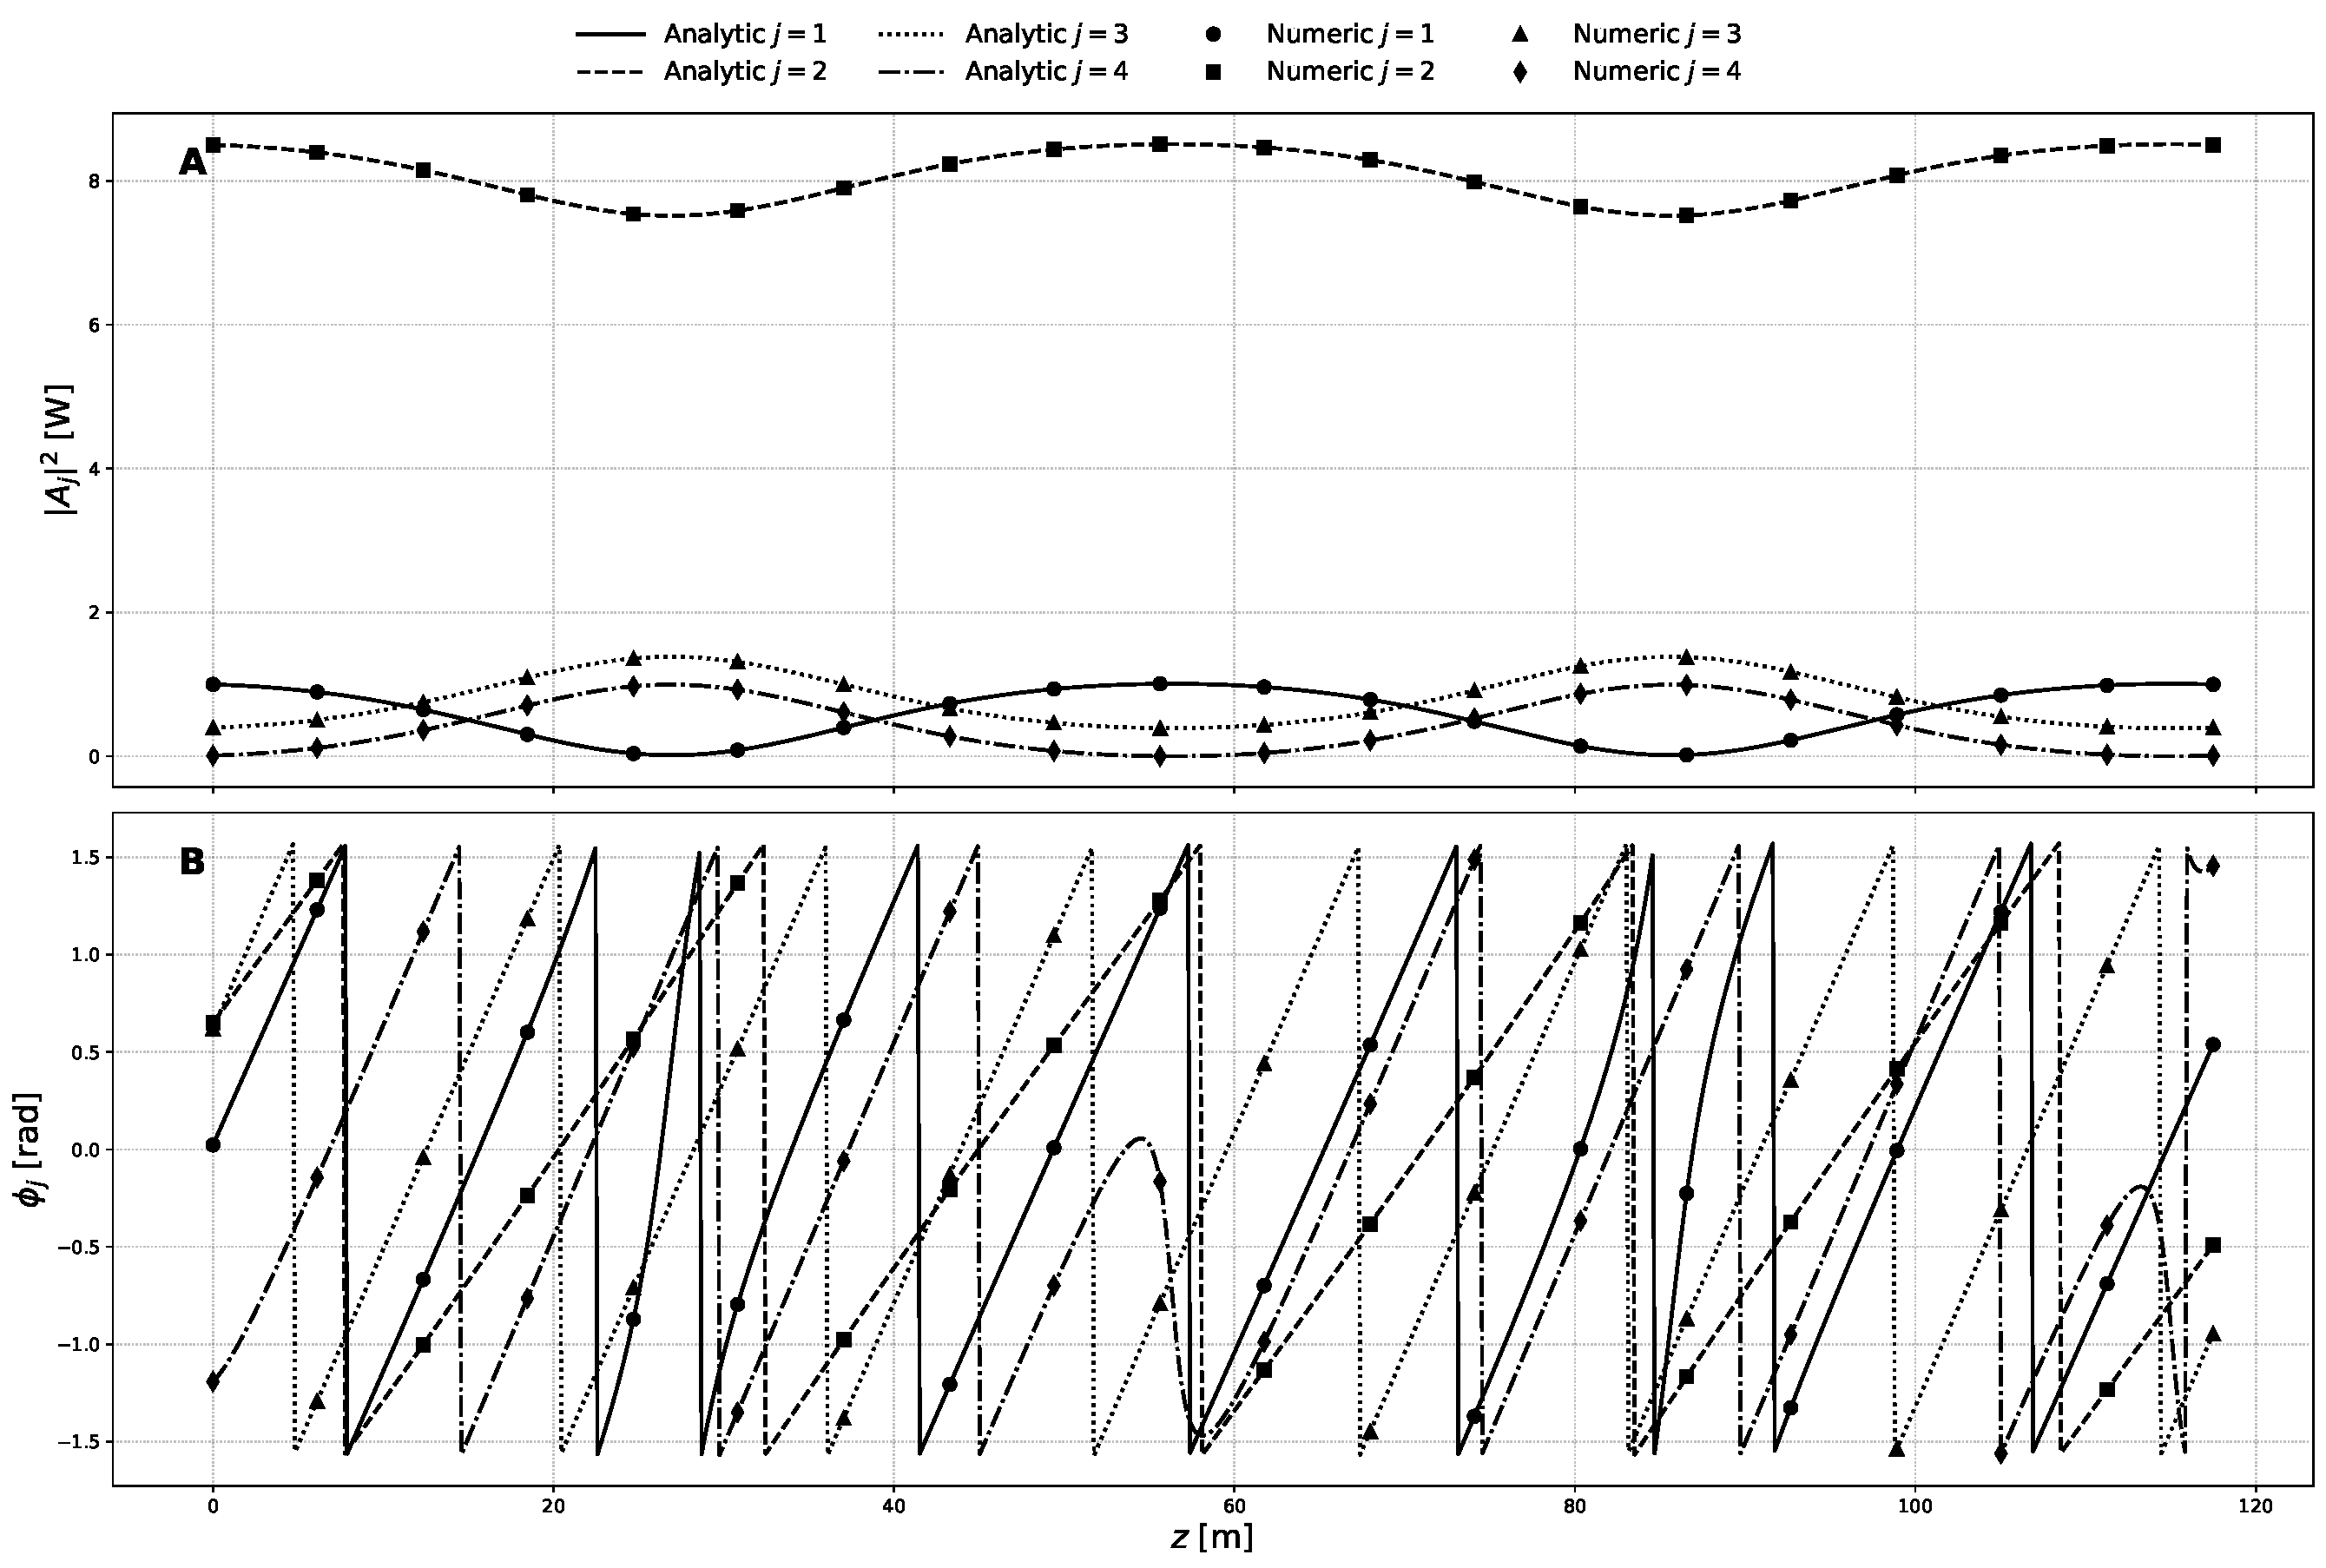
\includegraphics[width=1.0\textwidth]{plots/case2_plot_1.pdf}
\caption{\textbf{A} Intensity $\mathcal{P}_j=|A_j|^2$, and \textbf{B} phase $\phi_j$ of physical field amplitudes: analytic solution \eqref{eq:u-v-quartic} converted via \externaleqref{S-eq:u-v-A} (dashed lines) compared with numerical integration (symbols).}
\label{fig:case2-plot1}
\end{figure}

\subsection{Asymmetric coherent coupling}\label{cc:subsec:asymmetric-physical}

To test unequal coefficients on the physical slice, consider the normalised field equations
\begin{equation}
\frac{dA_j}{dz}=i\left(\beta_j+\sum_{k=1}^2G_{j,k}|A_k|^2\right)A_j+iA_{3-j},\qquad j=1,2,
\label{cc:eq:asymmetric-physical}
\end{equation}
with $\beta_1=0.3$, $\beta_2=-0.2$, $G_{1,1}=1.2$, $G_{2,2}=0.7$, and $G_{1,2}=G_{2,1}=0.25$.
The fields are mapped as in \externaleqref{S-cc:eq:uv-to-jensen}, with $a_1=-i\beta_1$, $a_2=i\beta_2$, $a_{j,j}=iG_{j,j}$ and $a_{1,2}=-iG_{1,2}$.
We take $A_1(0)=0.9+0.2i$ and $A_2(0)=0.3-0.1i$.
Figure~\ref{cc:fig:asymmetric-physical} compares the reconstructed optical powers and relative phase with direct integration of \eqref{cc:eq:asymmetric-physical} over $0\le z\le8$.
The maximum absolute error in either complex field at the 501 sampled points is $7.7\times10^{-13}$.
This example tests the generic unequal-self-phase case in a conservative physical system, with total power $0.95$ and both conjugation conditions preserved.

\begin{figure}[htbp]
\centering
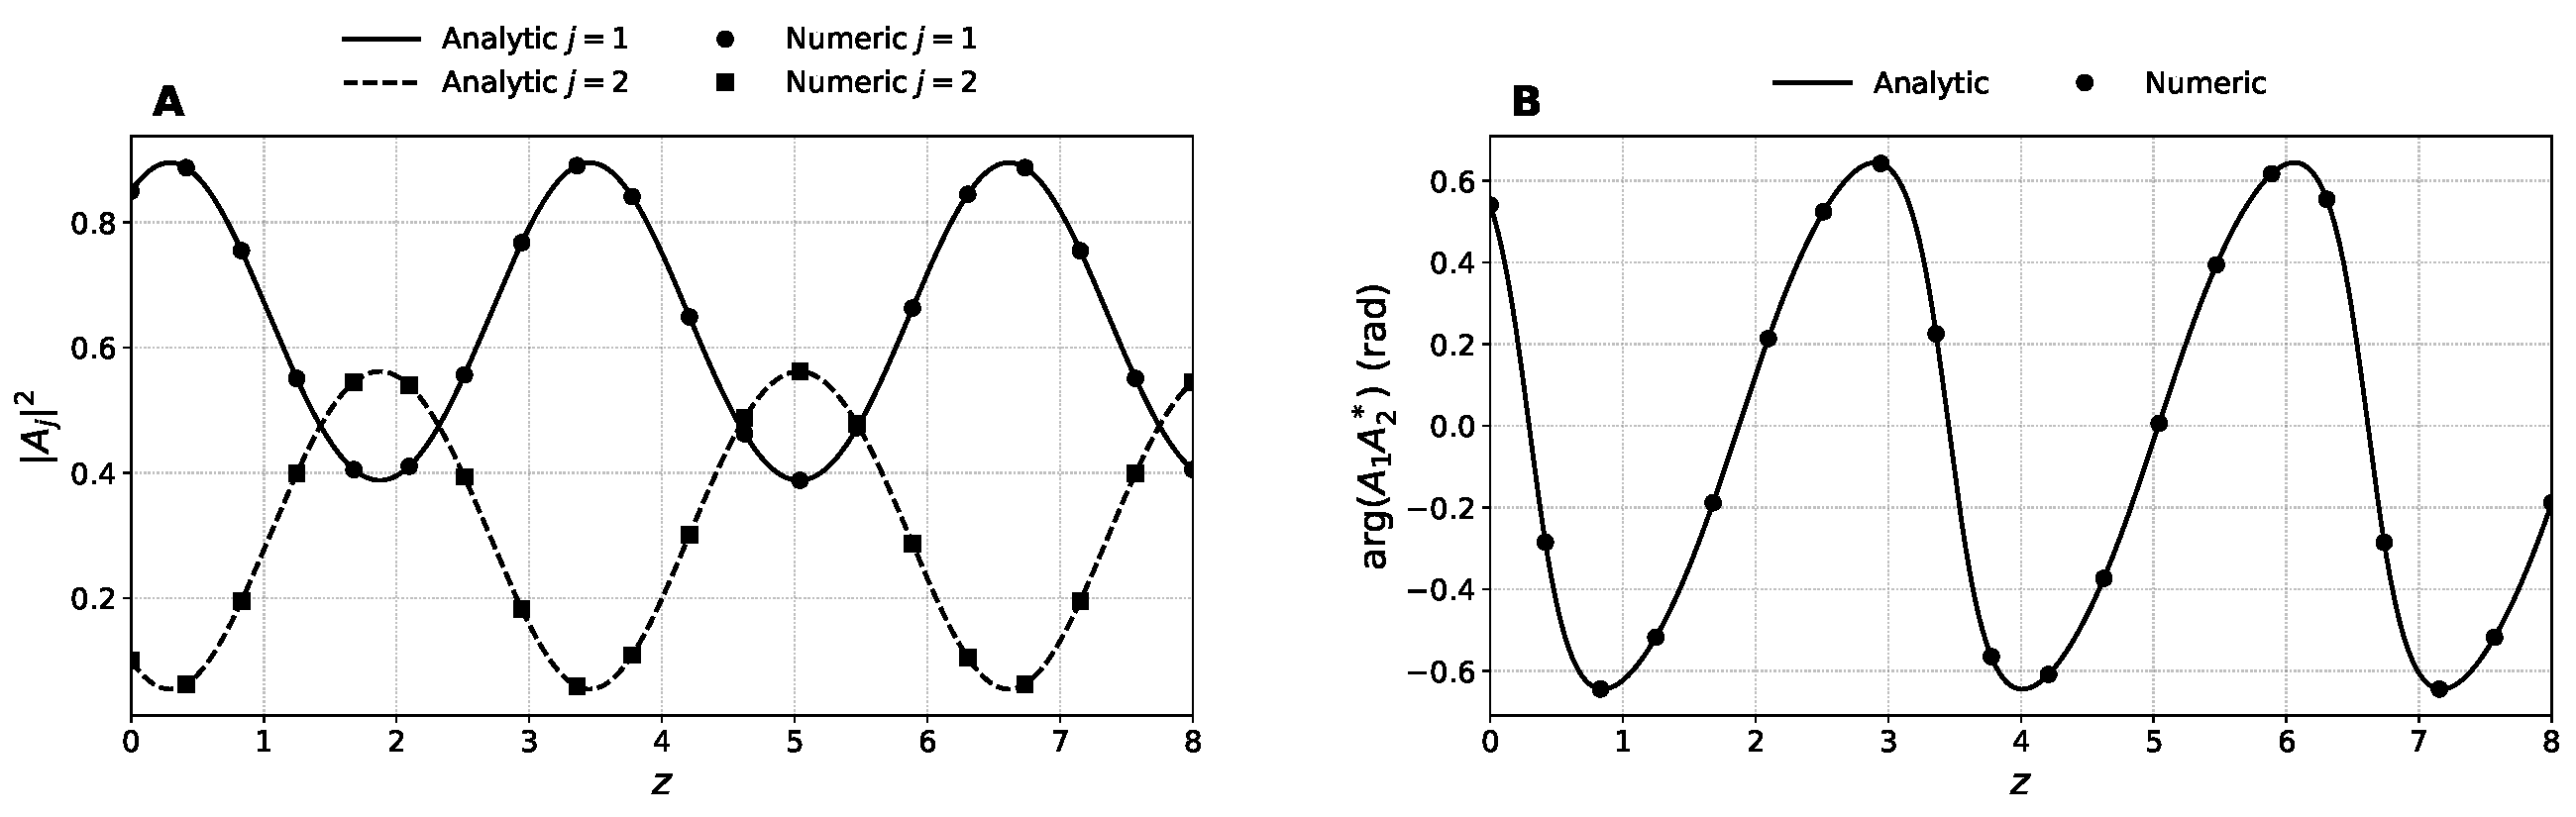
\includegraphics[width=\textwidth]{plots/coupler/asymmetric_physical.pdf}
\caption{An asymmetric conservative coupler: optical powers (left) and continuously unwrapped relative phase (right). Solid and dashed lines show the elliptic powers for modes 1 and 2; circles and squares show the corresponding direct numerical solutions. The relative phase uses a solid line and circles. Distance and power are normalised.}
\label{cc:fig:asymmetric-physical}
\end{figure}

\subsection{Numerical projection check}
We also integrate the three-mode degenerate-FWM equations generated by \eqref{cc:eq:Hbar-deg-fem} and, independently, the gauged coupler \eqref{cc:eq:uv-hat-system}, using initial data matched to the asymmetric example in Section~\ref{cc:subsec:asymmetric-physical}.
Applying the ratio map \eqref{cc:eq:projection-hat-as-bars} to the integrated FWM trajectory gives a maximum absolute discrepancy of $1.6\times10^{-12}$ across all four complex coupler components at 501 points over $0\le z\le8$.
With looser integration tolerances the discrepancy is $6.2\times10^{-11}$.
This checks the projection between independently evolved solutions, without evaluating the elliptic formulas; Supplement~1, Section~\ref*{S-supp:subsec:projection-numeric}, gives the matching data and tolerances.

\subsection{Additional checks}
The general complex FWM example and its figure are retained in Supplement~1, Section~\ref*{S-supp:sec:numerics}; its scale-normalised field discrepancy is approximately $2\times10^{-13}$.
The audits verify the full FWM transformation chain, the nonzero-$\Lambda_{1,j}$ cubic reconstruction for both coupling signs, all eight normal-form envelopes and all six lifted envelopes.
They also check the full ratio projection, its matched invariants and Hamiltonian, and the gauged Wronskians and Lam\'e potentials.

\FloatBarrier
\section{Conclusion}
We have reconstructed the FWM complex envelopes in Weierstrass form and identified their Baker--Akhiezer factors on a common elliptic curve.
The passage from conserved products through logarithmic derivatives to sigma functions makes zeros, poles, branching and exponential multipliers explicit, connecting optical envelope solutions to the functions of elliptic spectral theory.

This analytic visibility enables two applications to the complete mode equations.
Gauges and local normalisations remove the branching multipliers and transform generic quartic FWM trajectories to a parameter-free meromorphic system.
Total interaction degree four distinguishes the form-preserving cancellation in the power-exchange equation within the stated class of normalisations, and the full transformed interaction structure is established explicitly.
A degeneration with weights $(1,1,2)$ then supplies a three-mode FWM system whose ratio projection and inverse reciprocal gauge reconstruct the asymmetric-coupler envelopes.

Numerical comparisons and symbolic checks validate the reconstructed solutions, transformations and projection.
The Baker--Akhiezer representation thus supplies a common function-theoretic foundation for the envelope reconstruction and its two mode-level applications in nonlinear optics.

\begin{backmatter}
\bmsection{Acknowledgments} The author thanks Maria Dimou for a careful read of the manuscript.
\bmsection{Disclosures} The author declares no conflicts of interest.
\bmsection{Data availability} The symbolic derivations and numerical validation code supporting this work are available in Ref.~\cite{heskethFWMAndCouplerPaper}, including the original Jupyter notebooks with \emph{SymPy} derivations \cite{meurerSymPySymbolicComputing2017} and audit scripts. Additional formulas and numerical inputs are provided in Supplement~1.
\bmsection{AI declaration} GPT-6.1 Sol from OpenAI was used to assist with editing existing manuscript writing, and running numeric tests during development debugging.
\bmsection{Supplemental document} See Supplement~1 for supporting content.
\end{backmatter}

\bibliography{references}
\end{document}
